\documentclass[a4paper,14pt]{extarticle}

\usepackage[utf8x]{inputenc}
\usepackage[T1,T2A]{fontenc}
\usepackage[russian]{babel}
\usepackage{hyperref}
\usepackage{indentfirst}
\usepackage{here}
\usepackage{array}
\usepackage{graphicx}
\usepackage{caption}
\usepackage{subcaption}
\usepackage{chngcntr}
\usepackage{amsmath}
\usepackage{amssymb}
\usepackage{pgfplots}
\usepackage{pgfplotstable}
\usepackage[left=2cm,right=2cm,top=2cm,bottom=2cm,bindingoffset=0cm]{geometry}
\usepackage{multicol}

\renewcommand{\le}{\ensuremath{\leqslant}}
\renewcommand{\leq}{\ensuremath{\leqslant}}
\renewcommand{\ge}{\ensuremath{\geqslant}}
\renewcommand{\geq}{\ensuremath{\geqslant}}
\renewcommand{\epsilon}{\ensuremath{\varepsilon}}
\renewcommand{\phi}{\ensuremath{\varphi}}

\counterwithin{figure}{section}
\counterwithin{equation}{section}
\counterwithin{table}{section}
\newcommand{\sign}[1][5cm]{\makebox[#1]{\hrulefill}} % Поля подписи и даты
\graphicspath{{pics/}} % Путь до папки с картинками
\captionsetup{justification=centering,margin=1cm}
\def\arraystretch{1.3}

\usepackage{courier}

\usepackage{listings}
\lstset{ %
extendedchars=\true,
keepspaces=true,
language=C,						% choose the language of the code
basicstyle=\footnotesize,		% the size of the fonts that are used for the code
numbers=left,					% where to put the line-numbers
numberstyle=\footnotesize,		% the size of the fonts that are used for the line-numbers
stepnumber=1,					% the step between two line-numbers. If it is 1 each line will be numbered
numbersep=5pt,					% how far the line-numbers are from the code
backgroundcolor=\color{white},	% choose the background color. You must add \usepackage{color}
showspaces=false				% show spaces adding particular underscores
showstringspaces=false,			% underline spaces within strings
showtabs=false,					% show tabs within strings adding particular underscores
frame=single,           		% adds a frame around the code
tabsize=2,						% sets default tabsize to 2 spaces
captionpos=b,					% sets the caption-position to bottom
breaklines=true,				% sets automatic line breaking
breakatwhitespace=false,		% sets if automatic breaks should only happen at whitespace
escapeinside={\%*}{*)},			% if you want to add a comment within your code
postbreak=\raisebox{0ex}[0ex][0ex]{\ensuremath{\color{red}\hookrightarrow\space}},
texcl=true,
}

\lstset{basicstyle=\footnotesize\ttfamily,breaklines=true}

\begin{document}

\begin{titlepage}
\begin{center}
	\textbf{Санкт-Петербургский Политехнический Университет \\Петра Великого}\\[0.3cm]
	\small Институт компьютерных наук и технологий \\[0.3cm]
	\small Кафедра компьютерных систем и программных технологий\\[4cm]
	
	\textbf{ОТЧЕТ}\\ \textbf{о лабораторной работе}\\[0.5cm]
	\textbf{<<Использование стандартных подпрограмм для приближенного\\ вычисления интеграла>>}\\[0.1cm]
	\textbf{Вычислительная математика}\\[8.0cm]
\end{center}

\begin{flushright}
	\begin{minipage}{0.48\textwidth}
		\begin{flushleft}
			\small \textbf{Работу выполнил студент}\\[3mm]
			\small группа 23501/4 \hspace*{6mm} Дьячков В.В.\\[5mm]
			
			\small \textbf{Преподаватель}\\[5mm]
		 	\small \sign[3cm] \hspace*{5mm} к.т.н., доц. Цыган В.Н.\\[0.5cm]
		\end{flushleft}
	\end{minipage}
\end{flushright}

\vfill

\begin{center}
	\small Санкт-Петербург\\
	\small \the\year
\end{center}
\end{titlepage}

\section{Техническое задание}

\textbf{Вариант 7:} Для функции $f(x)$ по узлам $x_k$ построить интерполяционный полином Лагранджа $L(x)$ 10-й степени и сплайн функцию $S(x)$. Сравнить значения трех интегралов:

\begin{multicols}{3}
	\noindent 
	\[\int_0^3 f(x)dx\]
	\[\int_0^3 L(x)dx\]
	\[\int_0^3 S(x)dx\]
\end{multicols}

\section{Исходные данные}

Заданная функция: $f(x) = 1 - e^{-x}$

\vspace{0.5cm}

Узлы интерполяции: $x_k = 0.3 \cdot k\text{, для }k = 0, 1, ..., 10$

\section{Вычисление интегралов}

\subsection{Вычисление $\int f(x)dx$}

Аналитически найдем значение интеграла:
\vspace{-0.2cm}
\[
\int_0^3 f(x)dx = \int_0^3 \left(1 - e^{-x}\right) dx = \left.\left( x + e^{-x} \right)\right\vert_0^3 = 3 + e^{-3} - 1 \approx 2.04978706836786
\]

\subsection{Вычисление $\int L(x)dx$}

\makeatletter
\def\lst@PlaceNumber{\llap{\normalfont
                \lst@numberstyle{\the\lst@lineno}\kern\lst@numbersep}}
\makeatother

Для вычисления значения полинома Лагранджа в некоторой точке будем использовать подпрограмму \texttt{lagrange}:

\captionof{lstlisting}{main.cpp. Функция, вычисляющая значение полинома Лагранджа 10-ой степени в точке \texttt{x0}}
\lstinputlisting[label=code:hello_mod, linerange={21-23}]{comp_math/main_no_comments.cpp}
\parindent=1cm

Для вычисления интеграла $\int_0^3 L(x)dx$ будет использовать подпрограмму \texttt{quanc8}:

\captionof{lstlisting}{main.cpp. Параметры подпрограммы \texttt{quanc8}}
\lstinputlisting[label=code:hello_mod, linerange={54-60}]{comp_math/main_no_comments.cpp}
\parindent=1cm

\captionof{lstlisting}{main.cpp. Вызов подпрограммы \texttt{quanc8}}
\lstinputlisting[label=code:hello_mod, linerange={64-65}]{comp_math/main_no_comments.cpp}
\parindent=1cm

\subsection{Вычисление $\int S(x)dx$}

Для вычисления значения сплайн функции в некоторой точке будем использовать подпрограммы \texttt{spline} для нахождения векторов \texttt{B, C, D} и \texttt{seval} для вычисления значения сплайн функции:

\captionof{lstlisting}{main.cpp. Функция, вычисляющая значение сплайн функции в точке \texttt{x0}}
\lstinputlisting[label=code:hello_mod, linerange={26-38}]{comp_math/main_no_comments.cpp}
\parindent=1cm

Для вычисления интеграла $\int_0^3 S(x)dx$ будем использовать подпрограмму \texttt{quanc8}:

\captionof{lstlisting}{main.cpp. Параметры подпрограммы \texttt{quanc8}}
\lstinputlisting[label=code:hello_mod, linerange={54-60}]{comp_math/main_no_comments.cpp}
\parindent=1cm

\captionof{lstlisting}{main.cpp. Вызов подпрограммы \texttt{quanc8}}
\lstinputlisting[label=code:hello_mod, linerange={66-67}]{comp_math/main_no_comments.cpp}
\parindent=1cm

\section{Результаты}

На рисунке \ref{fig:res} показан результат выполнения программы. В таблице в первом столбце указаны значения независимой переменной (причем для проверки помимо заданных $x_k$ указаны и промежуточные значения), во втором -- значения исходной функции, в третьем -- значения полинома Лагранджа, а в последнем -- значения сплайн функции.

После таблицы приведены значения трех интегралов, вычисленные при помощи подпрограммы \texttt{quanc8}: $\int_0^3 f(x)dx$, $\int_0^3 L(x)dx$ и $\int_0^3 S(x)dx$. Можно заметить, что значения интеграла от исходной функции, вычсиленное аналитически, и значение интеграла, вычисленное с использованием подпрограммы \texttt{quanc8}, совпадают.

В качестве вспомогательной информации приведены разности между интегралом от исходной функции и интегралом от полинома Лагранджа и сплайн функции.

\begin{figure}[H]
\begin{center}
	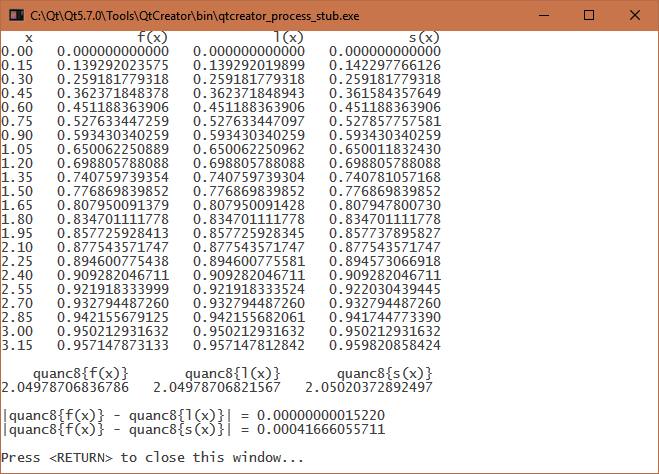
\includegraphics[width=0.95\textwidth]{screen_inversed}
	\caption{Результат выполнения программы}
	\label{fig:res}
\end{center}
\end{figure}

\section{Выводы}

По полученным результатам можно сделать вывод, что в данном случае лучше использовать полином Лагрнджа для приближенного вычисления интеграла $\int_0^3 f(x)dx$. 

\newpage

\section*{Приложение}

\captionof{lstlisting}{main.cpp}
\lstinputlisting[label=code:hello]{comp_math/main.cpp}
\parindent=1cm

\end{document}
